\chapter{Implementacija i korisničko sučelje}
		
		
		\section{Korištene tehnologije i alati}
		
			Kao dogovoren način razmjenjivanja ideja i dogovaranja oko projekta odabrana je 
			aplikacija Whatsapp \textbf{https://www.whatsapp.com/}. Github \textbf{https://github.com/}
			je odabran kao sustav za upravljanje cjelokupnim kodom projekta, a za izradu 
			svih dijagrama (sekvencijskih dijagrama, dijagrama razreda, dijagrama komponenti i sl.) 
			korišten je alat Visual Paradigm \textbf{https://online.visual-paradigm.com/}.
			
			Za razvojnu okolinu odabran je Visual Studio Code \textbf{https://code.visualstudio.com/}
			iz razloga što je jednostavan za korištenje jer pruža mogućnost pametnog dovršavanja
			na temelju vrsta varijabli i definicija funkcija za koju je zaslužan IntelliSense.
			Uz to sve, VSC je prilagodljiva okolina s puno ekstenzija, a i lako se povezuje 
			s GitHubom.
			
			Aplikacija je razvijena pomoću Java Spring Boot \textbf{https://spring.io/projects/spring-boot/},
			a korišten programski jezik je Java \textbf{https://www.java.com/en/}, verzija 17. 
			Za frontend je korišten programski jezik JavaScript \textbf{https://www.javascript.com/}, preciznije, 
			jezik TypeScript \textbf{https://www.typescriptlang.org/} koji je nadogradnja već
			postojećeg JavaScripta te biblioteka React \textbf{https://react.dev/}.
			Korištenjem TypeScripta omogućeno je dodavanje tipova i dodatnih mogućnosti nego samo
			koristeći JavaScript. Upotrebljena je i biblioteka ReactQuery koja omogućuje
			automatsko ažuriranje podataka - implementira logiku za osvježavanje i predmemoriranje 
			podataka, kao i za njihovu invalidaciju. Uz sve navedeno, korištene su i
			biblioteke UI komponenti ChakraUI i TailwindCSS za stiliziranje i dizajn korisničkog sučelja.
			
			Za bazu podataka korišten je Postgres \textbf{https://www.postgresql.org/} koja se 
			pokreće pomoću Dockera \textbf{https://www.docker.com/}, odnosno Docker containera.
			
			
			\eject 
		
	
		\section{Ispitivanje programskog rješenja}
			
			
			\subsection{Ispitivanje komponenti}
			\textit{Potrebno je provesti ispitivanje jedinica (engl. unit testing) nad razredima koji implementiraju temeljne funkcionalnosti. Razraditi \textbf{minimalno 6 ispitnih slučajeva} u kojima će se ispitati redovni slučajevi, rubni uvjeti te izazivanje pogreške (engl. exception throwing). Poželjno je stvoriti i ispitni slučaj koji koristi funkcionalnosti koje nisu implementirane. Potrebno je priložiti izvorni kôd svih ispitnih slučajeva te prikaz rezultata izvođenja ispita u razvojnom okruženju (prolaz/pad ispita). }
			
			
			
			\subsection{Ispitivanje sustava}
			
			Ispitivanje sustava izvedeno je u programskom jeziku Python koristeći Selenium WebDriver. Priloženi kodovi su u nastavku, ali prije toga je izdvojen zajednički kod koji koriste svi testovi.
			
			\begin{figure}[H]
				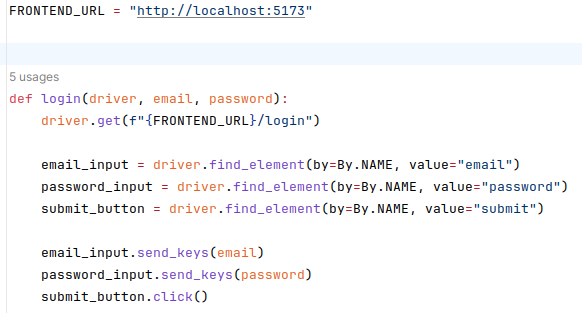
\includegraphics[width=\textwidth]{slike/selenium_common.png}
				\centering
				\caption{Zajednički kod testova}
				\label{fig:zajednicki-kod-testova}
			\end{figure}
			
			Prvi test ispituje pokušaj prijave s krivim podatcima. Očekivani je da se putanja ne promijeni te da se pojavi obavijest u obliku \textit{Toast}-a koja daje više informacija o greški.   
			
			\begin{figure}[H]
				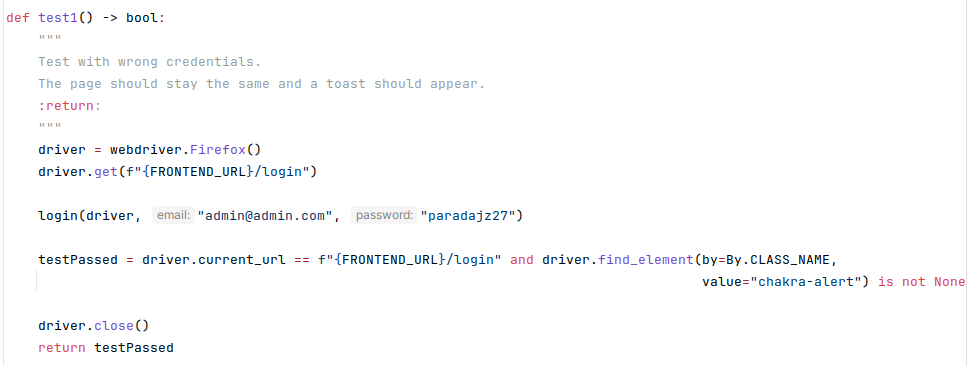
\includegraphics[width=\textwidth]{slike/selenium_test1.png}
				\centering
				\caption{Izvorni kod 1. testa}
				\label{fig:izvorni-kod-testa-1}
			\end{figure}
		
			Drugi test ispituje pokušaj prijave s ispravnim podatcima. Očekivano ponašanje je da se putanja promijeni te da gumb "Logout" bude vidljiv.
			
			\begin{figure}[H]
				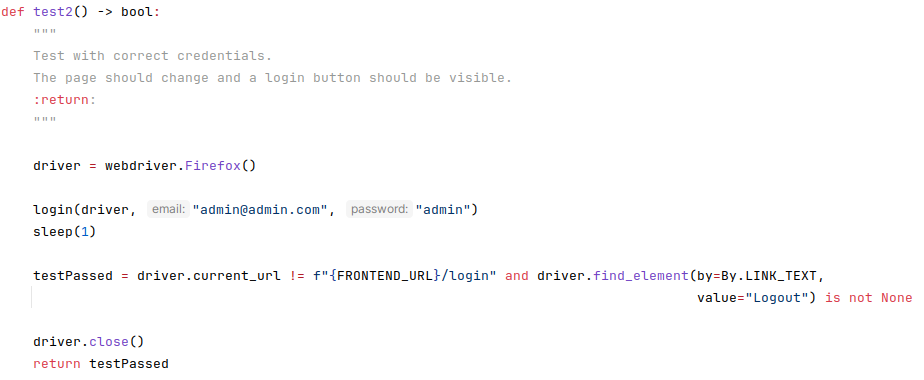
\includegraphics[width=\textwidth]{slike/selenium_test2.png}
				\centering
				\caption{Izvorni kod 2. testa}
				\label{fig:izvorni-kod-testa-2}
			\end{figure}
		
			Treći test ispituje stvaranje transportne kompanije. Očekivano ponašanje je povećanje broja redaka u tablici koja prikazuje transportne kompanije za 1.
		
			\begin{figure}[H]
				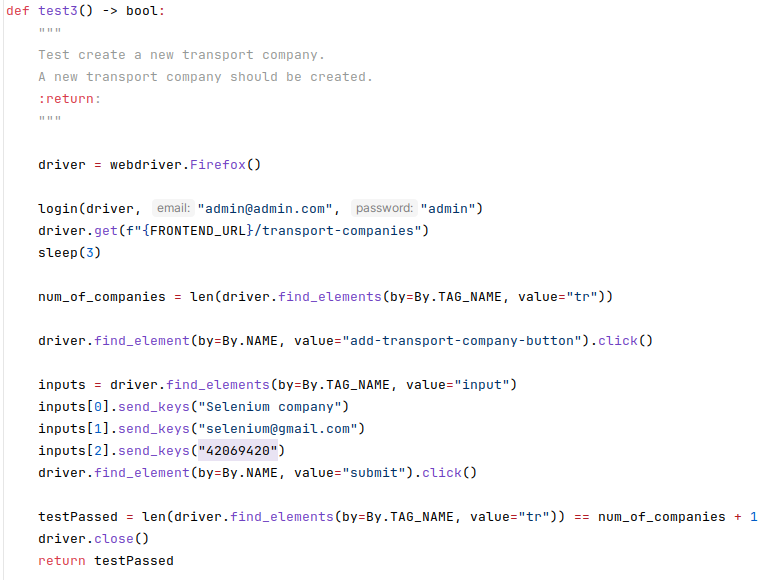
\includegraphics[width=\textwidth]{slike/selenium_test3.png}
				\centering
				\caption{Izvorni kod 3. testa}
				\label{fig:izvorni-kod-testa-3}
			\end{figure}
		
			Četvrti test ispituje brisanje transportne kompanije. Očekivano ponašanje je smanjenje broja redaka u tablici koja prikazuje transportne kompanije za 1
		
			\begin{figure}[H]
				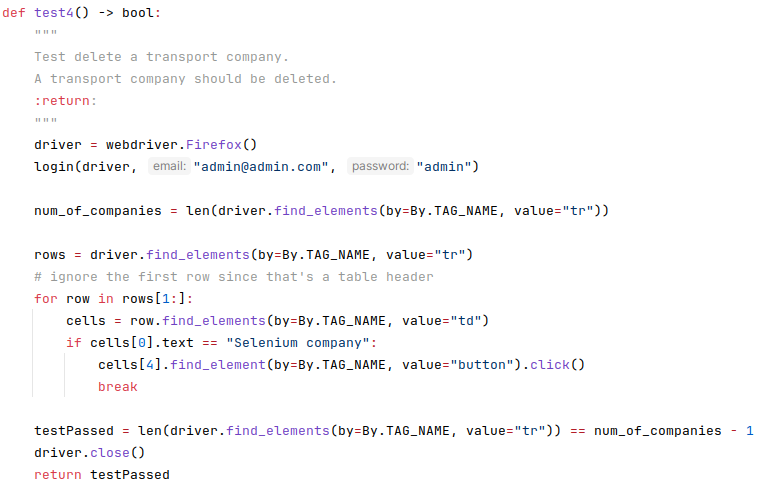
\includegraphics[width=\textwidth]{slike/selenium_test4.png}
				\centering
				\caption{Izvorni kod 4. testa}
				\label{fig:izvorni-kod-testa-4}
			\end{figure}
		
			Peti test ispituje odjavljivanje korisnika. Očekivano ponašanje je promjena putanje na "/login".
			
			\begin{figure}[H]
				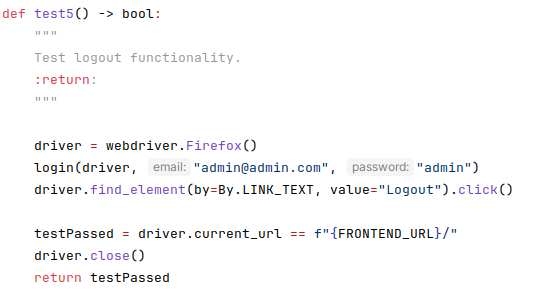
\includegraphics[width=\textwidth]{slike/selenium_test5.png}
				\centering
				\caption{Izvorni kod 5. testa}
				\label{fig:izvorni-kod-testa-5}
			\end{figure}
		
			Kod koji prikazuje kako su testovi pokrenuti.
			
			\begin{figure}[H]
				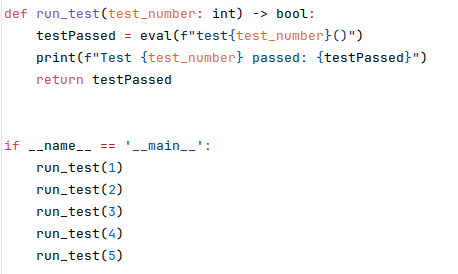
\includegraphics[width=\textwidth]{slike/selenium_running.png}
				\centering
				\caption{Izvršavanje testova}
				\label{fig:izvrsavanje-testova}
			\end{figure}
		
			Rezultati izvršenih testova.
			
			\begin{figure}[H]
				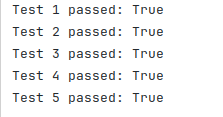
\includegraphics[width=\textwidth]{slike/selenium_results.png}
				\centering
				\caption{Rezultati testova}
				\label{fig:rezultati-testova}
			\end{figure}
				
			
			
			
			\eject 
		
		
		\section{Dijagram razmještaja}
			
			\textbf{\textit{dio 2. revizije}}
			
			 \textit{Potrebno je umetnuti \textbf{specifikacijski} dijagram razmještaja i opisati ga. Moguće je umjesto specifikacijskog dijagrama razmještaja umetnuti dijagram razmještaja instanci, pod uvjetom da taj dijagram bolje opisuje neki važniji dio sustava.}
			
			\eject 
		
		\section{Upute za puštanje u pogon}
		
			\textbf{\textit{dio 2. revizije}}\\
		
			 \textit{U ovom poglavlju potrebno je dati upute za puštanje u pogon (engl. deployment) ostvarene aplikacije. Na primjer, za web aplikacije, opisati postupak kojim se od izvornog kôda dolazi do potpuno postavljene baze podataka i poslužitelja koji odgovara na upite korisnika. Za mobilnu aplikaciju, postupak kojim se aplikacija izgradi, te postavi na neku od trgovina. Za stolnu (engl. desktop) aplikaciju, postupak kojim se aplikacija instalira na računalo. Ukoliko mobilne i stolne aplikacije komuniciraju s poslužiteljem i/ili bazom podataka, opisati i postupak njihovog postavljanja. Pri izradi uputa preporučuje se \textbf{naglasiti korake instalacije uporabom natuknica} te koristiti što je više moguće \textbf{slike ekrana} (engl. screenshots) kako bi upute bile jasne i jednostavne za slijediti.}
			
			
			 \textit{Dovršenu aplikaciju potrebno je pokrenuti na javno dostupnom poslužitelju. Studentima se preporuča korištenje neke od sljedećih besplatnih usluga: \href{https://aws.amazon.com/}{Amazon AWS}, \href{https://azure.microsoft.com/en-us/}{Microsoft Azure} ili \href{https://www.heroku.com/}{Heroku}. Mobilne aplikacije trebaju biti objavljene na F-Droid, Google Play ili Amazon App trgovini.}
			
			
			\eject 
